\documentclass[12pt, titlepage]{article}
\usepackage{float}
\usepackage{changepage}
\usepackage{fancyhdr}
\usepackage{booktabs}
\usepackage{tabularx}
\usepackage{hyperref}
\usepackage{graphicx}
\usepackage{titling}
\usepackage[utf8]{inputenc}
\usepackage{graphicx}
\usepackage{gensymb}
\usepackage{siunitx}
\graphicspath{{./images/}}
\usepackage{array}
\graphicspath{ {figures/} }

\hypersetup{
    colorlinks,
    citecolor=black,
    filecolor=black,
    linkcolor=blue,
    urlcolor=blue
}
\usepackage[round]{natbib}
\begin{document}

\title{
    System Verification \& Validation Plan for MobiCharged\\
    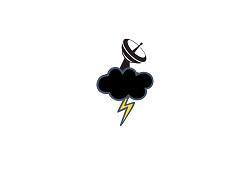
\includegraphics[width=9cm]{images/mobicharged.png} 
}
\author{Team Super Charged (No.33)
		\\ Nashit Mohammad - mohamn31
		\\ Eric Nguyen - nguyee13
		\\ Samuel De Haan - dehaas1
		\\ Eamon Earl - earle2
		\\ Mustafa Choueib - choueibm
}
    

\date{March 30, 2021, Rev. 1}


\maketitle

\pagenumbering{roman}
\tableofcontents
\listoffigures
\listoftables

\vspace{20pt}


\newpage

\pagenumbering{arabic}

\section{Revision History}
\begin{center}
\begin{table}[H]
\caption{\bf Revision History}
    \begin{tabular}{p{2cm}p{3cm}p{2cm}p{6cm}}
    \hline
    \bf Author & \bf Date & \bf Version & \bf Description\\
    \hline
    All & November 2nd, 2022 & Rev 0 & Created first draft of document\\
    \hline
    Nashit & March 30th, 2023 & Rev 1 & Corrected minor spelling and grammatical errors\\
    \hline
    Nashit & March 30th, 2023 & Rev 1 & Updated table 3 (verification \& validation team) to reflect changes and increase communication between project sectors\\
    \hline
    Nashit & March 31st, 2023 & Rev 1 & Updated table 4 (general plan for SRS verifications) to reflect changes\\
    \hline
    Nashit & March 31st, 2023 & Rev 1 & Updated system test descriptions to reflect changes and increase clarity \\
    \hline
    Nashit & March 31st, 2023 & Rev 1 & Linked references of system unit tests which will send reader to the unit test being discussed to lower the cognitive load of having to scroll down\\
    \hline
    Nashit & April 01st, 2023 & Rev 1 & Updated design verification plan and added a general checklist (table 5)\\
    \hline
    Nashit & April 01st, 2023 & Rev 1 & Updated reflection to incorporate information about specific group-mates\\
    \hline
    \end{tabular}
\end{table}
\end{center}



\section{General Information}
\subsection{Definitions}
\begin{table}[H]
\caption{\bf Naming Conventions and Terminology}
\begin{tabular}{ |p{6cm}|p{8cm}|  } 
 \hline
\bf Word & \bf Definition/Context\\
 \hline
 FR - Functional Requirement & Requirements that describe what the product is supposed to do\\
 \hline
NFR - Non-functional Requirement & Requirements that describe qualities that product will have\\
\hline
Data Smoothing & The process of using old data as well as "future" data in order to predict designs.\\
\hline
ML & "Machine Learning" algorithm.\\
\hline
SRS & Software Requirements Specification\\
\hline
Cryptography & The practice and study of techniques for secure communication\\
\hline
Asymmetric Key Cryptography & An encryption and decryption system that includes a public and private key pair\\
\hline
Functional Testing & Type of software testing that validates the software system against the functional requirements/specifications\\
\hline
Structural Testing & Type of software testing that uses the internal design of the software\\
\hline
Dynamic Testing & Test cases that are executed at run-time\\
\hline
Static Testing & Testing that does not require program execution\\
\hline
Manual Testing & Tests written and executed manually by team members\\
\hline
Automated Testing & Testing that makes use of software tools that execute tests automatically\\
\hline
System Testing & Testing that tests the system as a completed program and is based on the requirements\\
\hline
PROCESS-BENCHMARK & The average time required for completion of the current process (6 hours)\\
\hline
\end{tabular}
\end{table}

\subsection{Summary}
The construction industry is not only essential for the ever-growing infrastructure of our society but also a key factor used to determine the success in communities. With the Greater-Toronto-Area being one of the highest ranked increasing communities in regards to construction from across the globe, it is salient to ensure any buildings whether residential, commercial or industrial, are built with the highest of standard, highlight the importance of safety, and promote on-going innovation. 
\par
Engineers are tasked with design in construction to exceed requirements without hindering safety. Safety is a topic that is never missed within the industry and is continuously being highlighted amongst designs; especially as Engineers are reminded of their moral obligations to society by their awarded rings upon graduation. 
\par
As a current process, the construction industry places sensors within concrete spaces to continuously test and/or monitor the integrity of buildings during, as well as after construction. Ultimately however, these sensors run out of battery and are required to be re-charged. The industry still faces challenges when attempting to charge these sensors with the method of remote charging as the current products that satisfy remote charging abilities are yet to be optimized. There are a significant number of buildings being built in the Greater-Toronto-Area, which is emphasized considering that 70\% of cranes within Canada are in just the GTA alone. 
\par
To place innovation in the sub-field of safety within the industry, it is indeed a requirement to modernize the ability of producing efficient remote charging systems and to have the design process optimized to provide the most effective results. 
\par
MobiCharged aims to solve these gaps in the industry by producing a machine learning based software that aids these Engineers in designing remote charging systems based on their application requirements. Moreover, MobiCharged aims to produce a physical system that simulates a remote charging device for the purpose of demonstrations as well as applying real constraints pulled from the physical system onto the software.


\subsection{Objectives}
The objective in this document is to establish a plan meant to validate \& verify certain aspects of the system that correlate with the successful completion of satisfying requirements as well as ensuring the system is built as per intentions. The key objectives with this plan is to build confidence in the outputs produced by our system as well as establish confirmation of ease of navigation for our users when using our system. A selected key objective that should not be ignored is the aim to not only output application variables that will work successfully for the application, but to specifically output the most optimized solution. 

\subsection{Relevant Documents}
This Validation \& Verification Plan will highlight new plans revolving around testing. However, many components will overlap with previous published documents. The following are relevant documents that is suggested to be read in parallel with this report:
\begin{itemize}
    \item Hazard Analysis
    \item SRS Report
    \item Design Document
    \item PEP8 - Coding Style Guideline for Python
\end{itemize}


\section{Plan}

\subsection{Verification \& Validation Team}
Table 3 below highlights the team involved in the V\&V process as well as their respective roles.

\begin{center}
\begin{table}[H]
    \centering
    \begin{tabular}{|p{4cm}|p{9cm}|}
        \hline
        Team Member &  Role\\
        \hline
        Nashit & V\&V Team Lead - assigned the role of over-viewing the V\&V process \& delegating tasks to other members based on their respective schedules as well as integrating member’s tasks together. This role relays important information to the team\\
        \hline
        Eamon & Software Testing Designer - assigned the role of establishing the appropriate tests for certain units of the software system\\
        \hline
        Eric & Software Tester - assigned the role of working with the Software Testing Designer and performing the software tests while reporting the outputs\\
        \hline
        Samuel & Hardware Testing Designer - assigned the role of establishing the appropriate tests for certain units of the hardware system\\
        \hline
        Mustafa & Software Testing Designer - assigned the role of establishing the appropriate tests for certain units of the software system\\
        \hline
    \end{tabular}
    \caption{Verification \& Validation Team}
    \label{tab:my_label}
\end{table}
\end{center}
Although table 3 displays the key roles assigned to team members, these roles can be considered as fluid as the process is open to being adaptive based on future events to occur. Moreover, the role displays the key roles but excludes the minor roles assigned to members - for example, Nashit is the V\&V Team Lead but will also work closely with Samuel as a Hardware System Tester to test components. In addition, to prevent the occurrence of different testers being excluded from one another, the V\&V Team Lead will encourage communication between testers through the weekly meetings and be the bridge between communication.


\subsubsection{SRS Verification Plan}
To ensure the system satisfies what it was intended to, it will be verified in relation to the SRS document; in particular to section 9, Functional Architecture.
\par
The plan to verify the system with the documented SRS consists of a systematic approach as well as an open-ended feedback approach.
\par
For the systematic approach, the current plan is to create a checklist that highlights all the key requirements listed in the SRS. Note that some of the requirements are non-functional and cannot have a feasible systematic approach, but rather a user feedback selection.
\par
In regards to the open-ended feedback approach, the current steps for action is to simulate a demonstration as well as a program start-up / walk-through for the supervisor; MobilitePower, in order to receive their constructive feedback. This will be tied in with feedback provided from other students as well which will simulate feedback from users. 
\par
It shall be noted that the SRS Verification plan shall be referenced in parallel with the System Test Descriptions as both sections highlight the verification and the validations for requirements of the system. 
\par
Table 4 below highlights a checklist for the key components of the SRS Verifications. This table is adaptable and will continue to be updated as the project proceeds.
\newpage
\fancyhf{}
\fancyhead[C]{\thepage}
\renewcommand{\headrulewidth}{0pt}
\pagestyle{fancy}

\begin{center}
\begin{table}[H]
    \centering
    \begin{tabular}{|p{2cm}|p{5cm}|p{7cm}|}
    \hline
    SRS No. & SRS Description & General Plan for Verification\\
    \hline
    SR1 & ML Model must optimize inputs faster than existing process & Compile the average time it takes for the current process to generate solutions(i.e. the process which MobilitePower uses; Matlab Simulations). Use that as a bench-mark and test if the system can display outputs better or worse than the bench-mark\\
    \hline
    SR2 & ML Model must be able to develop “new” simulations based on previous models & Manually check the current data set the ML model contains. Enter inputs outside of that set limit and check if data smoothing occurs. Verify those outputs later to ensure those outputs are satisfactory as per NFR11\\
    \hline
    SR3 & ML Model must be able to encrypt optimized data before exporting & Have a software design tester test if the outputs are encrypted during the export process manually. The tester has the control to claim it is encrypted or not\\
    \hline
    HR1 & The system must be able to simulate a remote charging device by levitating a particle for at least 5 minutes & The hardware design tester will place a particle in the hardware capsule and using a stopwatch, time if the particle is able to levitate for a minimum of 5 minutes\\
    \hline
    HR2 & The system must be able to levitate the particles within 15 seconds & The hardware design tester will test the speed of which the device is able to levitate the particles\\
    \hline
    NFR8 & The system shall be understandable within an hour of use & The software design tester will test if the software is easily understood / can be navigated with ease within an hour of learning through the means of a user survey with the presumption that the user has previous knowledge regarding the device's variables\\
    \hline
    NFR9 & The system must compute optimal configuration within 6 hours & The software can display a “compilation time taken”. The software design tester can note the time it takes through a series of testing and highlight whether or not it is under 6 hours or over\\
    \hline
    NFR11 & The system must have a relative accuracy of 5\% compared to current Matlab simulation & The software design tester will compare the current data set and verify it with the system’s outputs\\
    \hline
    \end{tabular}
    \caption{General Plan for SRS Verifications}
    \label{tab:my_label}
\end{table}
\end{center}

\fancyhf{}
\fancyhead[C]{\thepage}
\renewcommand{\headrulewidth}{0pt}
\pagestyle{plain}


\subsection{Design Verification Plan}
The plan to verify the design of both the software system as well as the hardware system will revolve around reviews. These reviews shall include internal reviews from the V\&V Team, the supervisor, and external reviews from students. 
\par
A checklist has been generated in table 5 below which revolves around the non-functional requirements of the system that also aligns with the system design. These sections will include NFR3, NFR7, NFR8, NFR12 and NFR15 (all of which are referenced from the SRS Document). Verifications will include visual checks as well as tests which will be highlighted in the system test descriptions. 
\par 
Please note that this checklist shall be considered as fluid and is subject to change based on project developments - final results of the checklist will be highlighted in the V\&V Report. 

\begin{center}
\begin{table}[H]
    \centering
    \begin{tabular}{|p{5cm}|p{5cm}|}
    \hline
    Design Check & Description\\
    \hline
    Black Boxed Hardware & The hardware system is designed in a manner such that the non-relevant hardware components (from the perspective of the user) are hidden such as wires\\
    \hline
    Minimized Eye Strain & The software system will be designed in a manner such that the color scheme of the front end minimized eye strain. This will be done by methods described in the Design Document and checked by user survey which will be a rating selection from 1 to 5\\
    \hline
    Continuous Availability & System is available at all times\\
    \hline
    Quick Installation & System is designed such that the installation process takes within an hour\\
    \hline
    Operating System & System operates on both Windows \& MAC OS\\
    \hline
    \end{tabular}
    \caption{General Preliminary Checklist for Design Verification}
    \label{tab:my_label}
\end{table}
\end{center}

\subsection{V\&V Verification Plan}
The V\&V Verification Plan would be best implemented through the process of reviews and/or issues created. This will be done through preliminary grading, internal reviews, student reviews and supervisor’s revisions. Moreover, an internal check will be created to ensure that the V\&V Plan verifies all the requirements as well as all the unit tests. 

\subsection{Implementation Verification Plan}

The first step of our implementation in the verification process is the development of the long-term error analysis process for our machine learner, as outlined in Section 3.5. It is intended to have this done for our POC demo on Nov 21st, 2022 to accompany the machine learning algorithm. This is a continuous implementation to procedurally verify \hyperlink{SFRT-3Anchor}{SFRT-3}. At this point in time we can also ensure our condition \hyperlink{SFRT-1Anchor}{SFRT-1} holds, as we can test the performance even if the average output is relatively inaccurate.

Verification of \hyperlink{SFRT-4Anchor}{SFRT-4} will follow shortly, as the next step of the algorithm is adding the data-smoothing ‘initiative’ element. From there, we will develop the server element and implement the ETL tests, satisfying \hyperlink{SFRT-5Anchor}{SFRT-5}. 

Hardware development and the associated validation will take place parallel to these processes. However, once the correctness of the physical system is validated manually through the means discussed in the sections to come, readings from it to further validate and test our error in regards to \hyperlink{SFRT-3Anchor}{SFRT-3} will be used and the validation of the ‘pseudo-optimality’ of our machine learner will be implemented. The physical aspects of the phase array will also be used to set constraints on the ‘initiative’ aspect of the algorithm’s data-smoothing, and thus constrain the validating conditions of \hyperlink{SFRT-4Anchor}{SFRT-4}. 

We will spend the rest of our development time after this point adding elegance, safety, and performance boosts to the program, like implementing and verifying the correctness of our encryption tools, as discussed in \hyperlink{SFRT-2Anchor}{SFRT-2}.

We will be continuously performing deep code walk-throughs amongst the developers, to share context and verify across the team that our assumptions and constraints are correct and well-formed. We will also perform a system walk-through and demo with our supervisor, taking place once when our full cycle including the data smoothing ‘initiative’ is implemented and validated (\hyperlink{SFRT-4Anchor}{SFRT-4}), and a second time when the server system is created and validated (\hyperlink{SFRT-5Anchor}{SFRT-5}). This will be a higher-level view of the architecture and system communications, as well as what it achieves. At these checkpoints, we will also share the progression that our continuous error analysis shows, and thus communicate the accuracy of the machine learner over time. In addition, we will use these demos as an opportunity to validate certain NFRs with our supervisor, specifically those relating to the ease of use of the program.

\subsection{Automated Testing \& Verification Tools}
The method of verifying the improvement of the probability model in the learner is a constant process, and one that requires continuous usage and polling of our system data. For instance, we might store the inputs and optimal outputs provided by the simulation, and then ask the learner itself what its ‘pseudo-optimal’ output is. We can then calculate the relative error between them, and store that in a database; were we to graph these items, we’d expect a continuous decrease in this error as time goes on. The automation of this process relies less on any pre-built tools, and more so on integrating this concept of continuous progress checking into the operation cycle itself, and using a database to log the error (general DB tooling). Essentially, we have incredibly useful oracle-based validation in this case, and in our final system context model (client-server system with multiple personal devices running the simulations), we can have one device dedicated to polling and mapping this data, and can flag the operator if it notices consistently poor trends in the predictive model.

The second prong of the system that must be integrated with automatic verification and testing is the server stream and passage of data, such that we confirm that valid data is being passed and nothing else. This can be done using any number of ETL (extract, transform, and learn) testing libraries in Python, like the open source library Birgitta. We would implement these ETL verifiers end-to-end, to ensure the integrity of the passing data. This would ensure the predictive model would not be corrupted by false data batches, and protect against system crashes as well. 

For unit testing in our Python code, we’ll use PyTest, a commonly used library that has built in support for testing code validity as well as code coverage present in the tests. As with all self-respecting developer teams, we will collectively aim for full coverage and expect less. Many unit tests will also be used to verify the acceptance and passing of valid data. Additionally, we'll be using Pylint to enforce our formatting and readability standards.


\subsection{Software Verification Plan}
To verify that the software outputs the correct data as intended, we will apply checks with current available data. This verification process is the same in nature as NFR11 mentioned in table 4. 
\par
The current method in regards to creating solutions when designing remote charges devices revolves around Matlab simulations. Simulations are done by altering a vast amount of variables within the Matlab software. The simulations then outputs the desired variables necessary to maximize whichever variable is desired while noting constraints - similar to a continuous optimization problem where studies are done on finding the minimum and/or maximum (i.e. convex \& concave functions). 
\par
Since there were already simulations completed by MobilitePower, the supervisor will provide their current data for us to verify if our ML Method is effective, i.e. if our system outputs the same values that the simulation method does. 
\par
Moreover, another method for verifying our data is by doing routine checks (on values where we don’t currently have data on / currently have simulations done for). This can be done by applying the simulation method on arbitrary data sets and verifying that the simulation method and our ML method provide the same values given some tolerance. 
\par
Finally, the V\&V Team will work with the supervisor by holding demonstrations to ensure the scope is met and the system meets the requirements.

\section{System Test Description}
\subsection{Tests for Functional Requirements}
\subsubsection{Data Output}
\begin{enumerate}
    \hypertarget{SFRT-1Anchor}{}
    \item{SFRT-1\\}
    \textbf{Description:} This test will ensure the ML algorithm will determine the optimal solution in a shorter duration than the current process\\
    \textbf{Type:} Functional, Dynamic, Automated\\
    \textbf{Initial State:} Program is idle and awaiting required input\\
    \textbf{Input:} Desired remote charger configuration\\
    \textbf{Output:} Optimal remote charger solution along with the elapsed time to produce the optimal solution\\
    \textbf{How Test Will Be Performed:} A feasible (i.e. input that works theoretically based on mathematical constraints) configuration will be provided for testing. The ML algorithm will take the given input and produce the required and optimal output. The elapsed time that the algorithm takes to output the optimal solution will be compared to that of the PROCESS-BENCHMARK.This test will be performed on a Windows based OS computer in which the software is intended to run, as mentioned in the SRS. \\
    \textbf{Pass Condition:} Elapsed time $<$ PROCESS-BENCHMARK\\

    \hypertarget{SFRT-2Anchor}{}
    \item{SFRT-2\\}
    \textbf{Description:} This test will ensure that the exported data output is encrypted\\
    \textbf{Type:} Functional, Dynamic, Manual\\
    \textbf{Initial State:} ML program has computed the optimal solution\\
    \textbf{Input:} Optimal remote charger solution\\
    \textbf{Output:} An encrypted version of the optimal remote charger solution\\
    \textbf{How Test Will Be Performed:} The optimal remote charger solution will be computed and used for testing. Using this solution, the program must apply a public key to the data that is to be exported. This will convert the data into a format that will not be understandable to anyone who does not have the private key. This public and private key pairing is used in asymmetric key cryptography. The tester will then apply the private key to the encrypted data and ensure that the result matches the optimal solution. Testing to ensure that the data is not understandable will be done through the means of the tester who will have control on labelling it as a pass or a fail.\\
    \textbf{Pass Condition:} Exported Data (encrypted) = Optimal Solution $*$ Public key \&\& Optimal Solution = Exported Data (encrypted) $*$ Private Key\\
    
    \hypertarget{SFRT-3Anchor}{}
    \item{SFRT-3\\}
    \textbf{Description:} This test will ensure that the solution provided by the algorithm is optimized and correct\\
    \textbf{Type:} Functional, Dynamic, Manual\\
    \textbf{Initial State:} Program is idle and awaiting required input\\
    \textbf{Input:} A configuration in which the optimal solution has already been deduced\\
    \textbf{Output:} The optimal remote charger solution\\
    \textbf{How Test Will Be Performed:} A configuration that has already had the optimal solution deduced using the current process will be used. The algorithm will then produce the desired optimal solution which will be evaluated against the existing predetermined solution such that the error is within 5 percent\\
    \textbf{Pass Condition:} ML Algorithm Optimal Solution $=$ Predetermined Optimal Solution +/- 5 percent\\
\end{enumerate}

\subsubsection{Data Smoothing}
\begin{enumerate}
    \hypertarget{SFRT-4Anchor}{}
    \item{SFRT-4\\}
    \textbf{Description:} This test will ensure that the ML model can accurately and efficiently develop new simulations based on previous models\\
    \textbf{Type:} Functional, Dynamic, Manual\\
    \textbf{Initial State:} Program is idle and awaiting input\\
    \textbf{Input:} Desired configuration that does not exist in the current data set of the ML model\\
    \textbf{Output:} New data set that includes the previously trained models\\
    \textbf{How Test Will Be Performed:} The test will be performed by checking the existing data set that the ML model contains. Based on this, the input will be one that does not exist in the current data set. The program must then perform data smoothing and train itself based on the new input parameters and develop a new data set. Validity of the outputs of the new data set will be completed by SFRT-3\\
    \textbf{Pass Condition:} ML algorithm begins running new simulations using the new input parameters\\
\end{enumerate}

\subsubsection{Data Processing}
\begin{enumerate}
    \hypertarget{SFRT-5Anchor}{}
    \item{SFRT-5\\}
    \textbf{Description:} This test will ensure that the ML model can process incoming simulation data from multiple source devices\\
    \textbf{Type:} Functional, Dynamic, Manual\\
    \textbf{Initial State:} Program is in idle state\\
    \textbf{Input:} Simulation data from multiple devices\\
    \textbf{Output:} New ML Data set containing all newly received simulation data\\
    \textbf{How Test Will Be Performed:} The developers will run multiple simulations on different devices which will be used for this test. The data gathered from these simulations will be passed onto the ML algorithm which will then have to process and train the model using this data.\\
    \textbf{Pass Condition:} The ML model can correctly process and train itself using the simulation data coming from multiple source devices\\

    \item{SFRT-6\\}
    \textbf{Description:} This test will ensure that the ML model is able to interpret data exported directly from Matlab simulations\\
    \textbf{Type:} Functional, Dynamic, Manual\\
    \textbf{Initial State:} Program is in idle state and running simulations\\
    \textbf{Input:} Exported data from Matlab\\
    \textbf{Output:} New ML Data set containing the data from the Matlab simulation\\
    \textbf{How Test Will Be Performed:} A Matlab simulation will be run on the host device that the ML program is running on. Upon completion of the Matlab simulation, the data will be exported into a directory that the ML model will automatically access. The ML model will then process and interpret the data, and train itself using that data. This will ensure that the ML algorithm can properly interpret and access exported data from Matlab simulations, which will be verified manually by the tester who will authority to claim it as a pass or fail\\
    \textbf{Pass Condition:} ML algorithm properly interprets and accesses the data exported by Matlab and begins to train the model based on that data\\
\end{enumerate}

\subsubsection{Hardware System Functional Requirements}
\begin{enumerate}
    \item{HFRT-1\\}
    \textbf{Description:} This test will ensure the physical system is able to levitate a particle within the hardware capsule for at least 5 minutes\\
    \textbf{Type:} Functional, Static, Manual\\
    \textbf{Initial State:} Physical levitator (turned off) and particles within the hardware capsule\\
    \textbf{Input:} Physical levitator is turned on\\
    \textbf{Output:} Device begins to levitate particles\\
    \textbf{How Test Will Be Performed:} The tester will manually set up a blockade (paper) between the levitator and the particles. The amount of blockage between the two devices will be up to the discretion of the tester. Once set up, the tester will turn on the device and ensure the particles are levitating\\ 
    \textbf{Pass Condition:} The levitator will levitate the particles for 5 minutes\\

    \item{HFRT-2\\}
    \textbf{Description:} This test will ensure that the hardware system can levitate a particle within 15 seconds since its initial state\\
    \textbf{Type:} Functional, Static, Manual\\
    \textbf{Initial State:} OFF\\
    \textbf{Input:} System is turned ON\\
    \textbf{Output:} Particles levitate\\
    \textbf{How Test Will Be Performed:} The system will be off and a blockage (piece of paper) will be placed between the array of transistors and the particles (all within the hardware capsule). The system will then be turned on with the ideal case being that the particles then levitate. This test will also be done with HFRT-1\\
    \textbf{Pass Condition:} Time Required to Levitate Particles $<$ 15 Seconds\\
\end{enumerate}

\subsection{Tests for Non-Functional Requirements}

\subsubsection{Ease of Use}
\begin{enumerate}
    \item{SNFRT-1\\}
    \textbf{Description:} This test will ensure that the system is easy to use\\
    \textbf{Type:} Functional, Static, Manual\\
    \textbf{Initial State:} Program is in idle state\\
    \textbf{Input:} Users are asked to use the program and input a configuration to receive the optimal configuration\\
    \textbf{Output:} Users are able to retrieve an optimal configuration from the ML algorithm\\
    \textbf{How Test Will Be Performed:} The testers will gather a group of users and ask them to provide the program input and retrieve the optimal output produced by the algorithm\\
    \textbf{Pass Condition:} 80\% of users will successfully be able to provide input and retrieve the output within an hour of use\\

    \item{SNFRT-2\\}
    \textbf{Description:} This test will ensure that the system is easy to install\\
    \textbf{Type:} Functional, Static, Manual\\
    \textbf{Initial State:} The program is not installed on the test device\\
    \textbf{Input:} Program is provided via USB\\
    \textbf{Output:} Program is properly installed and launched\\
    \textbf{How Test Will Be Performed:} The user will be provided a USB stick containing the program. The user will then be instructed to install the program onto a device\\
    \textbf{Pass Condition:} 80\% of users will be able to successfully install and launch the program within an hour\\
\end{enumerate}

\subsubsection{Fault Tolerance}
\begin{enumerate}
    \item{SNFRT-3\\}
    \textbf{Description:} This test will ensure that the ML algorithm will be able to discard any corrupted data without adding it to the database\\
    \textbf{Type:} Functional, Dynamic, Manual\\
    \textbf{Initial State:} The program will be in the process of determining the optimal input\\
    \textbf{Input:} Tester will force close the program\\
    \textbf{Output:} The program will shut down\\
    \textbf{How Test Will Be Performed:} The tester will run the program for any valid input configuration for this test. While the program is determining the optimal solution for the given input, the tester will shutdown the program\\
    \textbf{Pass Condition:} The program will shutdown and discard the corrupted data without applying any changes to the existing database\\
\end{enumerate}

\subsubsection{Adaptability}
\begin{enumerate}
    \item{SNFRT-4\\}
    \textbf{Description:} This test will ensure that the program is applicable on Windows \& MAC OS\\
    \textbf{Type:} Functional, Dynamic, Manual\\
    \textbf{Initial State:} The application will be installed on different devices with different operating systems\\
    \textbf{Input:} The program is launched\\
    \textbf{Output:} The program is opened and is running successfully\\
    \textbf{How Test Will Be Performed:} The program will be provided on multiple different devices with different operating systems. The testers will then launch the program and ensure that it opens and runs successfully\\
    \textbf{Pass Condition:} Application opens without issue and is functional\\
\end{enumerate}

\subsubsection{Access Requirements}
\begin{enumerate}
    \item{SNFRT-5\\}
    \textbf{Description:} This test will be used to ensure that only authorized users can access the program\\
    \textbf{Type:} Functional, Dynamic, Manual\\
    \textbf{Initial State:} Log-in screen\\
    \textbf{Input:} Correct username and password combination\\
    \textbf{Output:} The program displays the home screen with access to functionality\\
    \textbf{How Test Will Be Performed:} The program will recognize specific log-in information. The tester will manually input this information and ensure that the program by-passes the initial log-in screen\\
    \textbf{Pass Condition:} Authorized user has access to the program functionality\\
\end{enumerate}

\subsection{Traceability Between Tests \& Requirements}

\begin{center}
\begin{table}[H]
    \centering
    \begin{tabular}{|p{2cm}|p{7cm}|}
    \hline
    \textbf{Test-ID} & \textbf{Associated Requirements}\\
    \hline
    SFRT-1 & SR1, NFR8\\
    \hline
    SFRT-2 & SR3, NFR16\\
    \hline
    SFRT-3 & SR4, NFR11\\
    \hline
    SFRT-4 & SR2\\
    \hline
    SFRT-5 & SR5, SR6\\
    \hline
    SFRT-6 & SR6\\
    \hline
    HFRT-1 & HR1\\
    \hline
    HFRT-2 & HR2\\
    \hline
    HFRT-3 & HR1, HR2\\
    \hline
    SNFRT-1 & NFR7, NFR3\\
    \hline
    SNFRT-2 & NFR8\\
    \hline
    SNFRT-3 & NFR13\\
    \hline
    SNFRT-4 & NFR15\\
    \hline
    SNFRT-5 & NFR4\\
    \hline
    \end{tabular}
    \caption{Traceability Between Tests \& Requirements}
    \label{tab:my_label}
\end{table}
\end{center}

\begin{center}
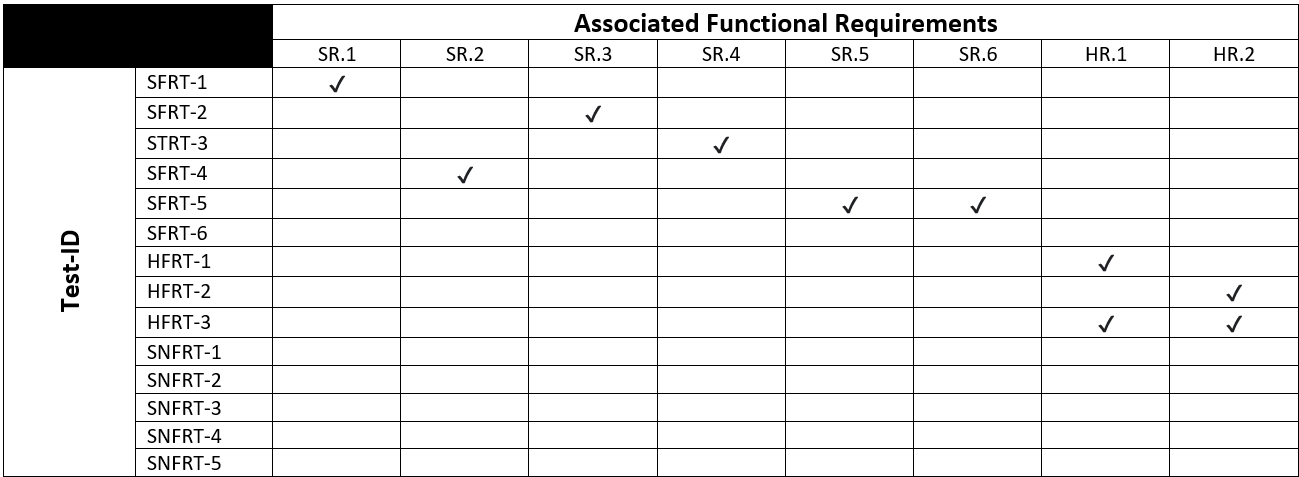
\includegraphics[width=16cm]{images/Traceability Matrix Functional Requirements.png}
\end{center}
\caption{Figure 1: Traceability Matrix for Functional Requirements \& Tests}

\begin{center}
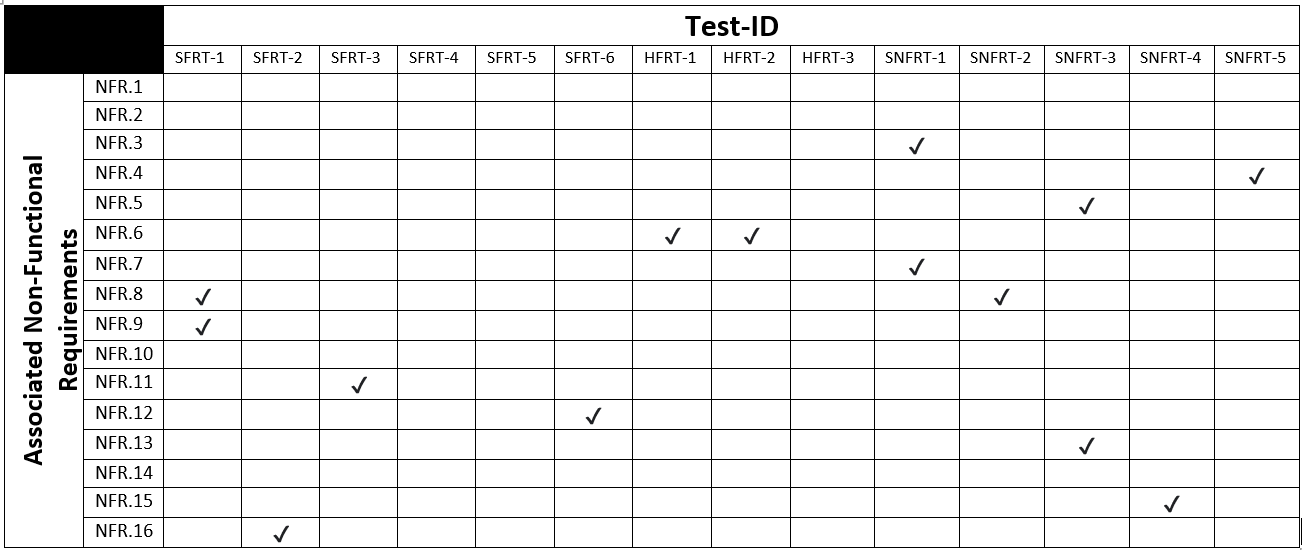
\includegraphics[width=16cm]{images/Traceability Matrix Non-Functional Requirements.png}
\end{center}
\caption{Figure 2: Traceability Matrix for Non-Functional Requirements \& Tests}


\section{Unit Test Description}
The unit test description is not applicable at this stage. This will be completed after the software has been completed for further evaluation.

\section{Appendix}

\subsection{Reflection}

\subsubsection{}

Part of the knowledge that the Software V&V team will need to acquire pertains to the performance of MobilitePower’s current optimization system. The current system will need to be understood and the performance characteristics of it quantified. SR1 and NFR11 are both related to the current system that is in place. Thus it must be understood and quantified so that verification of our product may be done. This will primarily be completed through communication with the supervisor as well as our team's bridge of communication with him which is assigned to Eamon. 

The Software Testing Designers will need to also acquire knowledge in the area of boundary testing. The SRS number that is in association with this is SR2. Knowledge and skills in boundary testing will need to be honed in order to successfully test and verify that the data smoothing works as intended. This will require the Software Test Designers to develop a knowledge of the system and boundary testing principles so that the limits of our application are pushed. This will be taken care of by Mustafa \& Eric who take responsibility in the testing of the code, as outlined in table 3. 

The V\&V lead will need to push their knowledge of project management skills and the correlation between the two aspects of our project (hardware and software). Project Management skills will be required to ensure all aspects are completed on schedule. As the lead of the V\&V team, knowledge of testing on both systems will be required. This will require the V&V team leader to have a firm understanding of both aspects. As outlined in table 3, Nashit will be overviewing the project in this regard. 

The Hardware V\&V team will need to acquire further knowledge on the functional characteristics desired from the supervisor. HR1 and HR2 will require the Hardware V&V team to identify the characteristics of the product that are required in order for verification of the device to pass. Samuel will work with Eamon in getting this information from the supervisor and will devising a plan accordingly.  

\subsubsection{}

The first knowledge area, pertaining to MobilitePower’s current optimization system, will be grown by taking the approach of an information interview. The Software V\&V team will conduct a detailed information interview with the supervisor in order to determine the metrics our system must hit in order to improve over the current standard. 

In order to gain more understanding in regards to boundary testing for the Software V\&V team, a dive into peer reviewed papers will be conducted. Extensive research will be conducted to determine how to sufficiently test boundary conditions in a way that may find faults in our system.

The V\&V lead will stay up to date with each ‘department’ within the team to ensure that they are aware of progress and any risks to the deadline. V\&V lead will arrange meetings as necessary to ensure they have a firm understanding of both systems and the V\&V process that is taking place.

The Hardware V\&V team will also conduct an information interview with the supervisor to determine appropriate values for verification. This will include, but is not limited to, time required for charge and appropriate level of obstruction between charging device and device to be charged. 


\section*{References}
We will be referring to documentations provided by Mobilite-Power, however, as of now there are no references to mention.




\end{document}

